%%%%%%%%%%%%%%%%%%%%%%%%%%%%%%%%%%%%%%%%%%%%%%%%%%%
%
%  New template code for TAMU Theses and Dissertations starting Fall 2012.  
%  For more info about this template or the 
%  TAMU LaTeX User's Group, see http://www.howdy.me/.
%
%  Author: Wendy Lynn Turner 
%
%%%%%%%%%%%%%%%%%%%%%%%%%%%%%%%%%%%%%%%%%%%%%%%%%%%

\documentclass[colorlinks=false,12pt]{report}
\renewcommand{\familydefault}{\rmdefault}
\usepackage[latin9]{inputenc}
\usepackage[letterpaper]{geometry}
\geometry{verbose,tmargin=1.25in,bmargin=1.25in,lmargin=1.4in,rmargin=1.15in}
\pagestyle{plain}
\usepackage[doublespacing]{setspace}
\usepackage{tocloft}
\usepackage[rm, tiny,center, compact]{titlesec}
\usepackage{indentfirst}
\usepackage{epstopdf}
\usepackage{graphicx,float,wrapfig}
\usepackage{etoolbox}
\usepackage{tocvsec2}
\usepackage[titletoc]{appendix}
\usepackage{appendix}
\usepackage{tamuconfig}
\usepackage[font=singlespacing]{caption}

% Hyperref setup below.  You should be able to get away with using uncommenting just the first line.
% \usepackage[hidelinks]{hyperref}

% if \usepackage[hidelinks]{hyperref} doesn't work try this.
% \usepackage{hyperref}  % Hidelinks is an option that removes link visiability.  TAMU Thesis Offices prefers to not see the links. But often doesn't work.  
% 
% \hypersetup{
%     colorlinks=true,
%     linkcolor=black,
%     citecolor=black,
%     filecolor=black,
%     urlcolor=black,
% }
%%%%%%%%  End of hyperref setup.  One of these two options should work, but my motto with hyperref is when in doubt, comment it out!

\begin{document}
\renewcommand{\tamumanuscripttitle}{Type in your default title here}
\renewcommand{\tamupapertype}{Dissertation}
\renewcommand{\tamufullname}{First Middle Lastname}
\renewcommand{\tamudegree}{Doctor of Philosophy}
\renewcommand{\tamuchairone}{Chair Name}
% Uncomment out the next line if you have co-chairs.  You will also need to edit the titlepage.tex file.
%\newcommand{\tamuchairtwo}{Additional Chair Name}
\renewcommand{\tamumemberone}{Committee Member1}
\newcommand{\tamumembertwo}{Committee Member2}
\newcommand{\tamumemberthree}{Committee Member3}
\renewcommand{\tamudepthead}{Department Head}
\renewcommand{\tamugradmonth}{December}
\renewcommand{\tamugradyear}{2012}
\renewcommand{\tamudepartment}{Department Name}


%%%%%%%%%%%%%%%%%%%%%%%%%%%%%%%%%%%%%%%%%%%%%%%%%%%
%
%  New template code for TAMU Theses and Dissertations starting Fall 2012.  
%  For more info about this template or the 
%  TAMU LaTeX User's Group, see http://www.howdy.me/.
%
%  Author: Wendy Lynn Turner 
%	 Version .9.2
%  Last updated 6/21/2012
%
%%%%%%%%%%%%%%%%%%%%%%%%%%%%%%%%%%%%%%%%%%%%%%%%%%%

%%%%%%%%%%%%%%%%%%%%%%%%%%%%%% 
%% TITLE PAGE
%% The values get updated automatically.  Please do not make changes to this file other than adding/deleting committee members where necessary.
%%%%%%%%%%%%%%%%%%%%%%%%%%%%%%

\providecommand{\tabularnewline}{\\}

%\makeatother

%\usepackage{babel}
%\begin{document}
\begin{titlepage}
\begin{center}
\MakeUppercase{\tamumanuscripttitle}
\vspace{4em}

A \tamupapertype

by

\MakeUppercase{\tamufullname}

\vspace{4em}

\begin{singlespace}

Submitted to the Office of Graduate Studies of \\
Texas A\&M University \\

in partial fulfillment of the requirements for the degree of \\
\end{singlespace}

\MakeUppercase{\tamudegree}
\par\end{center}
\vspace{2em}
\begin{singlespace}
\begin{tabular}{ll}
Approved by: & \tabularnewline
& \cr
% If you have Co-Chairs comment out the 'Chair of Committee' line below and uncomment the 'Co-Chairs of Committee' line.
Chair of Committee, & \tamuchairone\tabularnewline
%Co-Chairs of Committee, & \tamuchairone\tabularnewline & \tamuchairtwo\tabularnewline
Committee Members, & \tamumemberone\tabularnewline
 & \tamumembertwo\tabularnewline
 & \tamumemberthree\tabularnewline
Department Head, & \tamudepthead\tabularnewline

\end{tabular}
\end{singlespace}
\vspace{4em}

\begin{center}
\tamugradmonth \hspace{2pt} \tamugradyear

\vspace{3em}

Major Subject: \tamudepartment \par
\vspace{3em}
Copyright \tamugradyear
\par\end{center}
\end{titlepage}
\pagebreak{}




 % This is simply a file that formats and adds your titlepage, please do not edit this unless you have a specific need. .
\chapter*{ABSTRACT}
\addcontentsline{tic}{part}{ABSTRACT}
\pagestyle{plain}
\pagenumbering{roman}
\setcounter{page}{2}
\indent In this dissertation, advanced numerical methods for highly forward
peaked scattering deterministic calculations are devised, implemented, and
assessed. Since electrons interact with the surrounding environment through
Coulomb interactions, the scattering kernel is highly forward-peaked. 
This bears the consequence that, with standard preconditioning, the standard Legendre
expansion of the scattering kernel requires too many terms for the discretized
equation to be solved efficiently using a deterministic method. The Diffusion
Synthetic Acceleration (DSA), usually used to speed up the calculation when
the scattering is weakly anisotropic, is inefficient for electron transport.
This led Morel and Manteuffel to develop an one-dimensional angular multigrid
(ANMG) which has proved to be very effective when the scattering is highly
anisotropic. Later, Pautz et al. generalized this scheme to multidimensional
geometries, but this method had to be stabilized by a diffusive filter that
degrades the overall convergence of the iterative scheme. In this dissertation, we
recast the multidimensional angular multigrid method without the filter as a
preconditioner for a Krylov solver. This new method is stable independently of
the anisotropy of the scattering and is increasingly more effective and
efficient as the anisotropy increases compared to DSA preconditioning wrapped
inside a Krylov solver. At the coarsest level of ANMG, a DSA step is needed. In
this research, we use the Modified Interior Penalty (MIP) DSA. This DSA was
shown to be always stable on triangular cells with isotropic scattering. 
Because this DSA discretization leads to symmetric definite-positive matrices, 
it is usually solved using a conjugate gradient preconditioned (CG) by SSOR but
here, we show that algebraic multigrid methods are vastly superior than more common
CG preconditioners such as SSOR.

Another important part of this dissertation is dedicated to transport 
equation and diffusion solves on arbitrary polygonal meshes. The advantages of
polygonal cells are that the number of unknowns needed to mesh a domain can be
decreased and that adaptive mesh refinement implementation is simplified:
rather than handling hanging nodes, the adapted computational mesh includes 
different types of polygons. Numerical examples are presented for arbitrary
quadrilateral and polygonal grids.
\pagebreak{}

\chapter*{DEDICATION}
\addcontentsline{toc}{part}{DEDICATION}

\indent aaa

\pagebreak{}

%%%%%%%%%%%%%%%%%%%%%%%%%%%%%%%%%%%%%%%%%%%%%%%%%%%
%
%  New template code for TAMU Theses and Dissertations starting Fall 2012.  
%  For more info about this template or the 
%  TAMU LaTeX User's Group, see http://www.howdy.me/.
%
%  Author: Wendy Lynn Turner 
%	 Version 1.0 
%  Last updated 8/5/2012
%
%%%%%%%%%%%%%%%%%%%%%%%%%%%%%%%%%%%%%%%%%%%%%%%%%%%


%%%%%%%%%%%%%%%%%%%%%%%%%%%%%%%%%%%%%%%%%%%%%%%%%%%%%%%%%%%%%%%%%%%%%%
%%                           ACKNOWLEDGEMENTS
%%%%%%%%%%%%%%%%%%%%%%%%%%%%%%%%%%%%%%%%%%%%%%%%%%%%%%%%%%%%%%%%%%%%%
\chapter*{ACKNOWLEDGEMENTS}
\addcontentsline{toc}{chapter}{ACKNOWLEDGEMENTS}  % Needs to be set to part, so the TOC doesnt add 'CHAPTER ' prefix in the TOC.


\indent Lorem ipsum dolor sit amet, consectetur adipiscing elit. Integer lectus quam, condimentum quis bibendum eu, sollicitudin eget lacus. Praesent non sodales odio. Class aptent taciti sociosqu ad litora torquent per conubia nostra, per inceptos himenaeos. Nulla ac luctus sapien. Morbi cursus sapien eget lorem fermentum hendrerit. Nam ac erat dui, in cursus velit. Vivamus hendrerit porttitor nisi, ut porttitor lorem volutpat eget. In ligula ligula, euismod ut condimentum sit amet, pulvinar sit amet diam. Pellentesque interdum, ipsum ullamcorper consequat dignissim, sem arcu egestas mauris, vitae interdum sem tortor ut ante. Nunc blandit laoreet nisi, non rutrum lorem hendrerit quis. Cras nunc diam, convallis et feugiat at, auctor id libero. Nunc facilisis massa eu eros imperdiet vestibulum. Vestibulum ante ipsum primis in faucibus orci luctus et ultrices posuere cubilia Curae; Donec non velit vitae tortor blandit semper.

Etiam vitae dolor nulla. Ut eros odio, rhoncus eget placerat vitae, elementum ac ante. Proin vitae odio eu nisl pharetra mattis. Pellentesque habitant morbi tristique senectus et netus et malesuada fames ac turpis egestas. Phasellus fermentum lacus consectetur neque consequat ullamcorper. Cras blandit urna non dui consequat molestie. Curabitur viverra nibh at nisi semper faucibus. Nam egestas mauris a enim dignissim nec consectetur tortor rutrum. Mauris at nisi in est luctus congue ut mattis est. Ut pretium, mi quis elementum cursus, ante eros suscipit ligula, ut porttitor elit leo sed turpis. Nam sed dui ligula.


\pagebreak{}
\chapter*{NOMENCLATURE}
\addcontentsline{toc}{part}{NOMENCLATURE}

\begin{xtabular}{ll}
      AGMG & AGgregation-based algebraic MultiGrid \tabularnewline
       AMG & Algebraic MultiGrid method \tabularnewline
       AMR & Adaptive Mesh Refinement method \tabularnewline
      ANMG & ANgular multigrid method \tabularnewline
  ANMG-DSA & ANMG using DSA at the coarsest level \tabularnewline
 ANMG-$P1$ & ANMG using $P1$SA at the coarsest level \tabularnewline
         B & Boltzmann \tabularnewline
       BFP & Boltzmann-Fokker-Planck \tabularnewline
       BLD & BiLinear Discontinuous finite elements \tabularnewline
         c & scattering ratio \tabularnewline
        CG & Conjugate Gradient method \tabularnewline
  $\bs{D}$ & directions-to-moments \tabularnewline
       DSA & Diffusion Synthetic Acceleration \tabularnewline
        FP & Fokker-Planck \tabularnewline
       GLC & Gauss-Legendre-Chebyshev \tabularnewline
     GMRES & Generalized Minimal RESidual method \tabularnewline
  $\bs{L}$ & streaming matrix \tabularnewline
  $\bs{M}$ & moments-to-directions matrix \tabularnewline
       MIP & Modified Interior Penalty \tabularnewline
       MIS & Maximally Independent Sets \tabularnewline
        ML & MultiLevel package of Trilinos \tabularnewline
        MM & Morel and Manteuffel angular multigrid method \tabularnewline
    $P1$SA & $P1$ Synthetic Acceleration \tabularnewline
     $P_l$ & Legendre polynomial of degree $l$ \tabularnewline
   $P_l^m$ & Associated Legendre polynomial of degree $l$ and order $m$
  \tabularnewline
       PAM & Pautz, Adams, and Morel angular multigrid method \tabularnewline
     PAMNF & PAM with No Filtering \tabularnewline
      PWLD & PieceWise Linear Discontinuous finite elements \tabularnewline
  $\tilde{R}$ & mean square stopping power \tabularnewline
       $S$ & restricted stopping power \tabularnewline
  $\tilde{S}$ & stopping power \tabularnewline
        SI & Source Iteration \tabularnewline
     $S_n$ & Discrete ordinates method of order $n$ \tabularnewline
     $SGS$ & Symmetric Gauss-Seidel \tabularnewline
       SPD & Symmetric Positive-Definite \tabularnewline
      SSOR & Symmetric Successive OverRelaxation method \tabularnewline
       $T$ & half of the restricted momentum transfer \tabularnewline
$\tilde{T}$ & half of the momentum transfer \tabularnewline
   $Y_l^m$ & spherical harmonic of degree $l$ and order $m$ \tabularnewline 
     $\bo$ & $(\mu,\varphi)$ unit vector in the flight direction \tabularnewline
     $\mu$ & $\cos(\theta)$ \tabularnewline
   $\mu_0$ & $\bo'\cdot \bo$ \tabularnewline
    $\psi$ & angular flux \tabularnewline
$\bs{\Sigma}$ & scattering cross sections matrix \tabularnewline
$\Sigma_a(\br,E)$ & absorption macroscopic cross section \tabularnewline
$\Sigma_s(\br,E)$ & scattering macroscopic cross section \tabularnewline
$\Sigma_s(\br,\bo'\cdot\bo,E'\rightarrow E)$ & differential scattering macroscopic 
  cross section \tabularnewline
$\Sigma_t(\br,E)$ & total macroscopic cross section \tabularnewline
  $\theta$ & directional polar angle \tabularnewline
 $\varphi$ & directional azimuthal angle \tabularnewline
\end{xtabular}

\pagebreak{}

%%%%%%%%%%%%%%%%%%%%%%%%%%%%%%%%%%%%%%%%%%%%%%%%%%%
%
%  New template code for TAMU Theses and Dissertations starting Fall 2012.  
%  For more info about this template or the 
%  TAMU LaTeX User's Group, see http://www.howdy.me/.
%
%  Author: Wendy Lynn Turner 
%	 Version 1.0 
%  Last updated 8/5/2012
%
%%%%%%%%%%%%%%%%%%%%%%%%%%%%%%%%%%%%%%%%%%%%%%%%%%%
%%%%%%%%%%%%%%%%%%%%%%%%%%%%%%%%%%%%%%%%%%%%%%%%%%%%%%%%%%%%%%%%%%%%%%
%%       TABLE OF CONTENTS
%%%%%%%%%%%%%%%%%%%%%%%%%%%%%%%%%%%%%%%%%%%%%%%%%%%%%%%%%%%%%%%%%%%%%
\phantomsection
\addcontentsline{toc}{chapter}{TABLE OF CONTENTS}  % Needs to be set to part, so the TOC doesnt add 'CHAPTER ' prefix in the TOC.
\begin{singlespace}
\renewcommand\contentsname{\normalfont} {\centerline{TABLE OF CONTENTS}}

%\setcounter{tocdepth}{4} % This puts \subsubsection[]{×} in your List of Tables.  The default is 3.


%%%%%%%%%%%%%  Adds Page above the page number in TOC
\setlength{\cftaftertoctitleskip}{1em}
\renewcommand{\cftaftertoctitle}{%
\hfill{\normalfont {Page}\par}}



\tableofcontents

\end{singlespace}

\pagebreak{}

%%%%%%%%%%%%%%%%%%%%%%%%%%%%%%%%%%%%%%%%%%%%%%%%%%%%%%%%%%%%%%%%%%%%%%
%%                           lIST OF FIGURES
%%%%%%%%%%%%%%%%%%%%%%%%%%%%%%%%%%%%%%%%%%%%%%%%%%%%%%%%%%%%%%%%%%%%%

\phantomsection
\addcontentsline{toc}{chapter}{LIST OF FIGURES}  % Needs to be set to part, so the TOC doesnt add 'CHAPTER ' prefix in the TOC.

\renewcommand{\cftloftitlefont}{\center\normalfont\MakeUppercase}

\setlength{\cftbeforeloftitleskip}{-12pt} %% Positions the LOF title vertically to match the chapter titles

\renewcommand{\cftafterloftitleskip}{12pt}
\renewcommand{\cftafterloftitle}{%
\\[\baselineskip]\mbox{}\hfill{\normalfont Page}}

\begingroup


\begin{center}
\begin{singlespace}
%% These values make the lof table entries appear double spaced between.
\setlength{\cftbeforechapskip}{0.4cm}
\setlength{\cftbeforesecskip}{0.30cm}
\setlength{\cftbeforesubsecskip}{0.30cm}
\setlength{\cftbeforefigskip}{0.4cm}
\setlength{\cftbeforetabskip}{0.4cm}
\listoffigures

\end{singlespace}
\end{center}
\pagebreak{}


%%%%%%%%%%%%%%%%%%%%%%%%%%%%%%%%%%%%%%%%%%%%%%%%%%%%%%%%%%%%%%%%%%%%%%
%%                           lIST OF TABLES
%%%%%%%%%%%%%%%%%%%%%%%%%%%%%%%%%%%%%%%%%%%%%%%%%%%%%%%%%%%%%%%%%%%%%%
%
\phantomsection
\addcontentsline{toc}{chapter}{LIST OF TABLES}  % Needs to be set to part, so the TOC doesnt add 'CHAPTER ' prefix in the TOC.

\renewcommand{\cftlottitlefont}{\center\normalfont\MakeUppercase}

\setlength{\cftbeforelottitleskip}{-12pt} %% Positions the LOF title vertically to match the chapter titles

\renewcommand{\cftafterlottitleskip}{12pt}
\renewcommand{\cftafterlottitle}{%
\\[\baselineskip]\mbox{}\hfill{\normalfont Page}}

\begin{center}
\begin{singlespace}

%% These values make the lot table entries appear double spaced between.
\setlength{\cftbeforechapskip}{0.4cm}
\setlength{\cftbeforesecskip}{0.30cm}
\setlength{\cftbeforesubsecskip}{0.30cm}
\setlength{\cftbeforefigskip}{0.4cm}
\setlength{\cftbeforetabskip}{0.4cm}
\listoftables

\end{singlespace}
\end{center}
\endgroup
\pagebreak{}  % Need this for the pagenumbering to be correct.   % This is simply a file that formats and adds your toc, lof, and lot, please do not edit this unless you have a specific need. .

%%%%%%%%%%%%%%%%%%%%%%%%%%%%%%%%%%%%%%%%%%%%%%%%%%%
%
%  New template code for TAMU Theses and Dissertations starting Fall 2012.  
%  For more info about this template or the 
%  TAMU LaTeX User's Group, see http://www.howdy.me/.
%
%  Author: Wendy Lynn Turner 
%	 Version 1.0 
%  Last updated 8/5/2012
%
%%%%%%%%%%%%%%%%%%%%%%%%%%%%%%%%%%%%%%%%%%%%%%%%%%%

%%%%%%%%%%%%%%%%%%%%%%%%%%%%%%%%%%%%%%%%%%%%%%%%%%%%%%%%%%%%%%%%%%%%%%
%%                           SECTION I
%%%%%%%%%%%%%%%%%%%%%%%%%%%%%%%%%%%%%%%%%%%%%%%%%%%%%%%%%%%%%%%%%%%%%


\pagestyle{plain} % No headers, just page numbers
\pagenumbering{arabic} % Arabic numerals
\setcounter{page}{1}


\chapter{\uppercase {Introduction: The Importance of Research}}
%%%%%%%%%%%%%%%%%%%%%%%%%%%%%%%%%%%%%%%%%%%%%%%%%%%%%%
\begin{figure}[H]
\centering
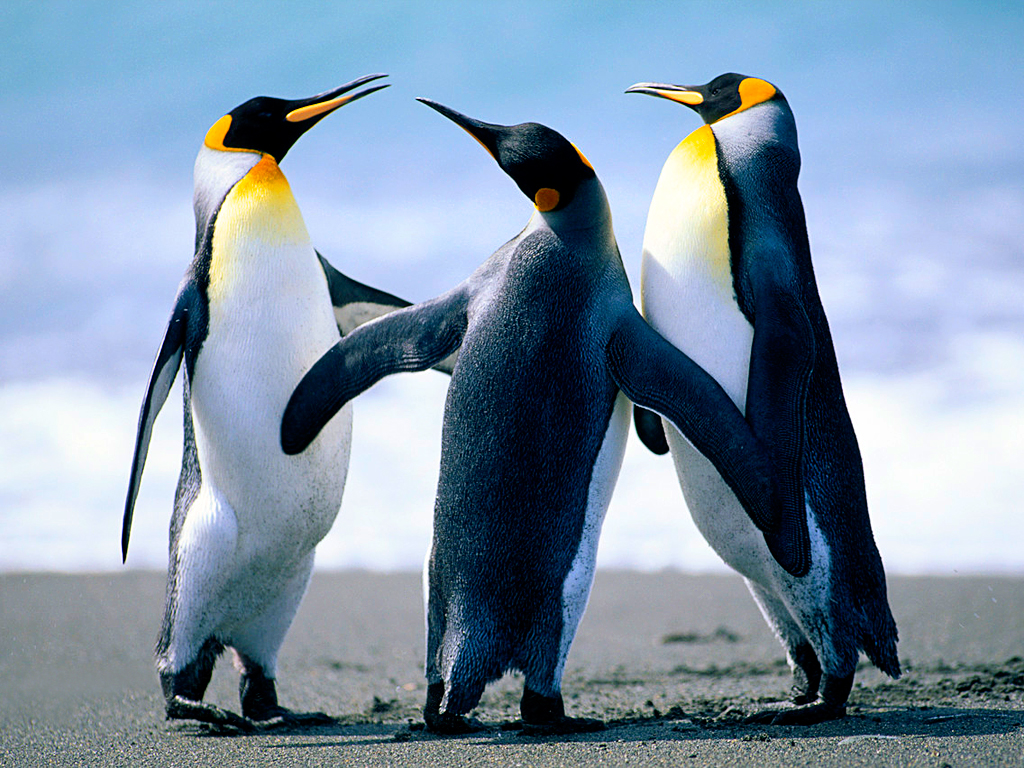
\includegraphics[scale=.50]{figures/Penguins.jpg}
\caption{TAMU figure - This is an example of a long figure title.  Figure titles need to be single-spaced within and double spaced between in the list of figures.}
\label{fig:tamu-fig1}
\end{figure}
%%%%%%%%%%%%%%%%%%%%%%%%%%%%%%%%%%%%%%%%%%%%%%%%%%%%%%

Text goes here.

\section{This is a Very Long Section Title This is a Very Long Section Title This is a Very Long Section Title }

More text here goes here.

\subsection{This is a Very Long Subsection Title This is a Very Long Subsection Title}

More text
\subsection{Subsection}

Subsection text

\section{Another Section}

Section text

%%%%%%%%%%%%%%%%%%%%%%%%%%%%%%%%%%%%%%%%%%%%%%%%%%%
%
%  New template code for TAMU Theses and Dissertations starting Fall 2012.  
%  For more info about this template or the 
%  TAMU LaTeX User's Group, see http://www.howdy.me/.
%
%  Author: Wendy Lynn Turner 
%	 Version 1.0 
%  Last updated 8/5/2012
%
%%%%%%%%%%%%%%%%%%%%%%%%%%%%%%%%%%%%%%%%%%%%%%%%%%%

%%%%%%%%%%%%%%%%%%%%%%%%%%%%%%%%%%%%%%%%%%%%%%%%%%%%%%%%%%%%%%%%%%%%%%%
%%%                           SECTION II
%%%%%%%%%%%%%%%%%%%%%%%%%%%%%%%%%%%%%%%%%%%%%%%%%%%%%%%%%%%%%%%%%%%%%%

\chapter{\uppercase {Literature Review: The Importance of Research Part Two- This is designed to test long titles in the TOC}}

Text goes here.

\section{New Section}
%%%%%%%%%%%%%%%%%%%%%%%%%%%%%%%%%%%%%%%%%%%%%%%%%%%%%%
\begin{figure}[H]
\centering
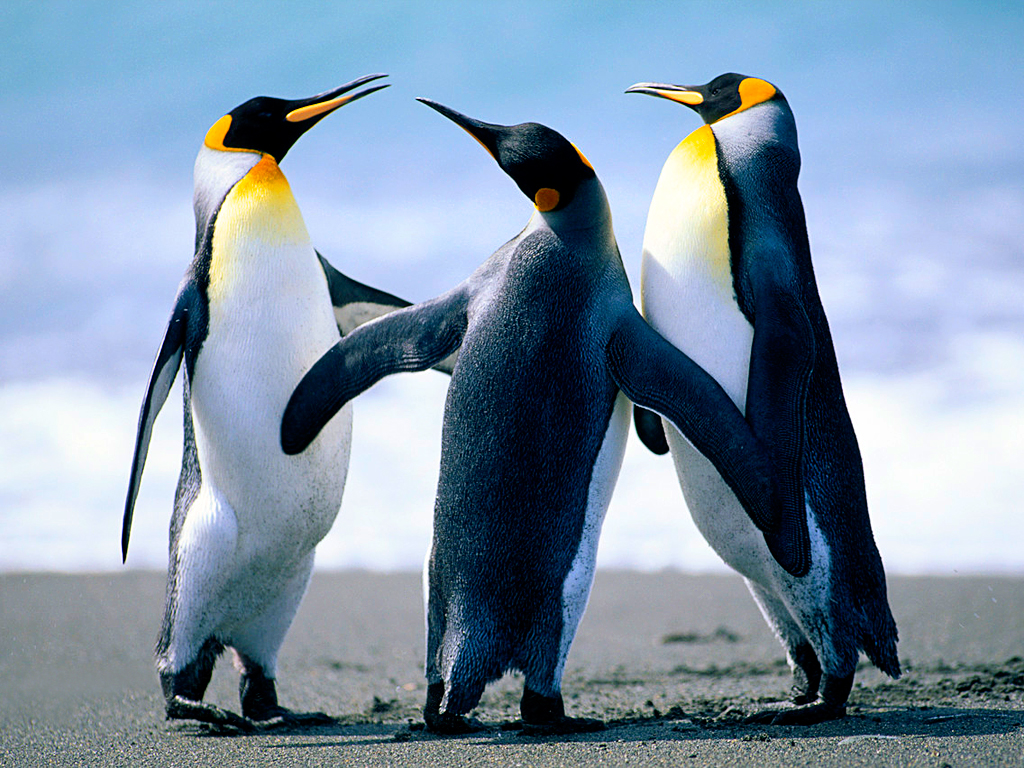
\includegraphics[scale=.50]{figures/Penguins.jpg}
\caption{TAMU figure}
\label{fig:tamu-fig2}
\end{figure}
%%%%%%%%%%%%%%%%%%%%%%%%%%%%%%%%%%%%%%%%%%%%%%%%%%%%%%
\subsection{Subsection}
\begin{table}[H]
\centering
\caption{This is a table template - This is an example of a long table title.  Table titles need to be single-spaced within and double spaced between in the list of tables.}
\begin{tabular}{|l|c|c|c|c|c|}
\hline
Product & 1 & 2 & 3 & 4 & 5\\
\hline
Price & 124.- & 136.- & 85.- & 156.- & 23.-\\
Guarantee [years] & 1 & 2 & - & 3 & 1\\
Rating & 89\% & 84\% & 51\% & & 45\%\\
\hline
\hline
Recommended & yes & yes & no & no & no\\
\hline
\end{tabular}
\label{tab:template1}
\end{table}


\subsection{Subsection}
%%%%%%%%%%%%%%%%%%%%%%%%%%%%%%%%%%%%%%%%%%%%%%%%%%%%%%
\begin{figure}[H]
\centering
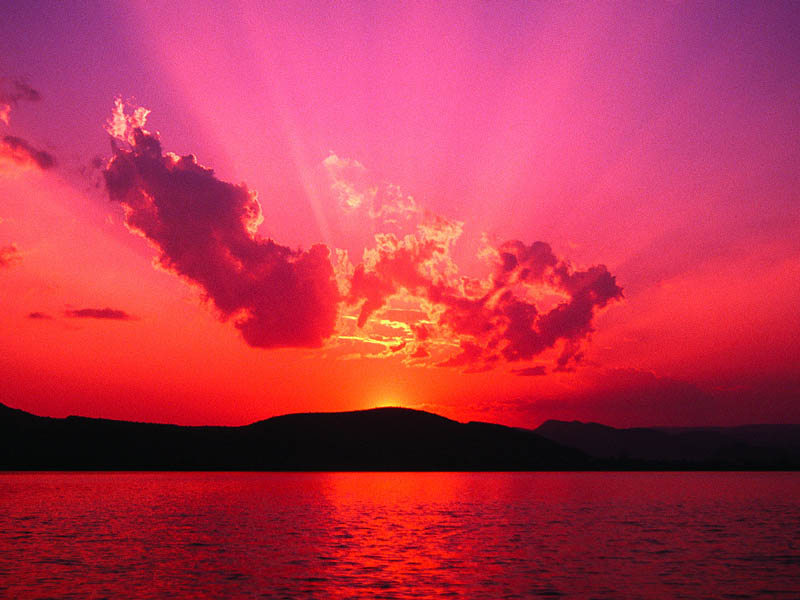
\includegraphics[scale=.50]{figures/Sunset.jpg}
\caption{Sunset figure}
\label{fig:sunset-fig2}
\end{figure}
%%%%%%%%%%%%%%%%%%%%%%%%%%%%%%%%%%%%%%%%%%%%%%%%%%%%%%
\subsubsection{This is a subsubsection}
\begin{table}[H]
\centering
\caption{This is a table template - This is an example of a long table title.  Table titles need to be single-spaced within and double spaced between in the list of tables.}
\begin{tabular}{|l|c|c|c|c|c|}
\hline
Product & 1 & 2 & 3 & 4 & 5\\
\hline
Price & 124.- & 136.- & 85.- & 156.- & 23.-\\
Guarantee [years] & 1 & 2 & - & 3 & 1\\
Rating & 89\% & 84\% & 51\% & & 45\%\\
\hline
\hline
Recommended & yes & yes & no & no & no\\
\hline
\end{tabular}
\label{tab:template1-2}
\end{table}
\section{Another Section}

%%%%%%%%%%%%%%%%%%%%%%%%%%%%%%%%%%%%%%%%%%%%%%%%%%%
%
%  New template code for TAMU Theses and Dissertations starting Fall 2012.  
%  For more info about this template or the 
%  TAMU LaTeX User's Group, see http://www.howdy.me/.
%
%  Author: Wendy Lynn Turner 
%	 Version 1.0 
%  Last updated 8/5/2012
%
%%%%%%%%%%%%%%%%%%%%%%%%%%%%%%%%%%%%%%%%%%%%%%%%%%%
%%%%%%%%%%%%%%%%%%%%%%%%%%%%%%%%%%%%%%%%%%%%%%%%%%%%%%%%%%%%%%%%%%%%%%
%%                           SECTION III
%%%%%%%%%%%%%%%%%%%%%%%%%%%%%%%%%%%%%%%%%%%%%%%%%%%%%%%%%%%%%%%%%%%%%



\chapter{\uppercase{Last Chapter: The Importance of Research}}

Text goes here \cite{Agrawal1986}.

\section{New Section}

%%%%%%%%%%%%%%%%%%%%%%%%%%%%%%%%%%%%%%%%%%%%%%%%%%%%%%
\begin{figure}[H]
\centering
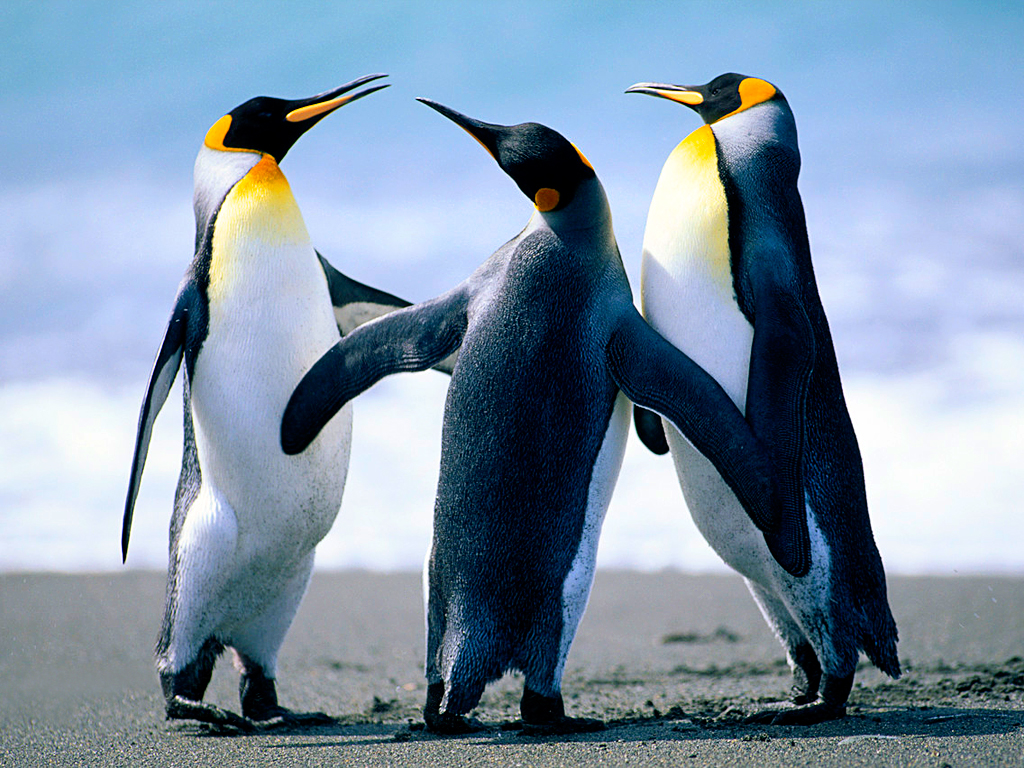
\includegraphics[scale=.50]{figures/Penguins.jpg}
\caption{TAMU figure}
\label{fig:tamu-fig3}
\end{figure}
%%%%%%%%%%%%%%%%%%%%%%%%%%%%%%%%%%%%%%%%%%%%%%%%%%%%%%
\section{Another Section}

Text between the figures.  Text between the figures. Text between the figures. Text between the figures.  Text between the figures. Text between the figures. Text between the figures.  Text between the figures. Text between the figures. Text between the figures.  Text between the figures. Text between the figures.
%%%%%%%%%%%%%%%%%%%%%%%%%%%%%%%%%%%%%%%%%%%%%%%%%%%%%%%
%\begin{figure}[H]
%\centering
%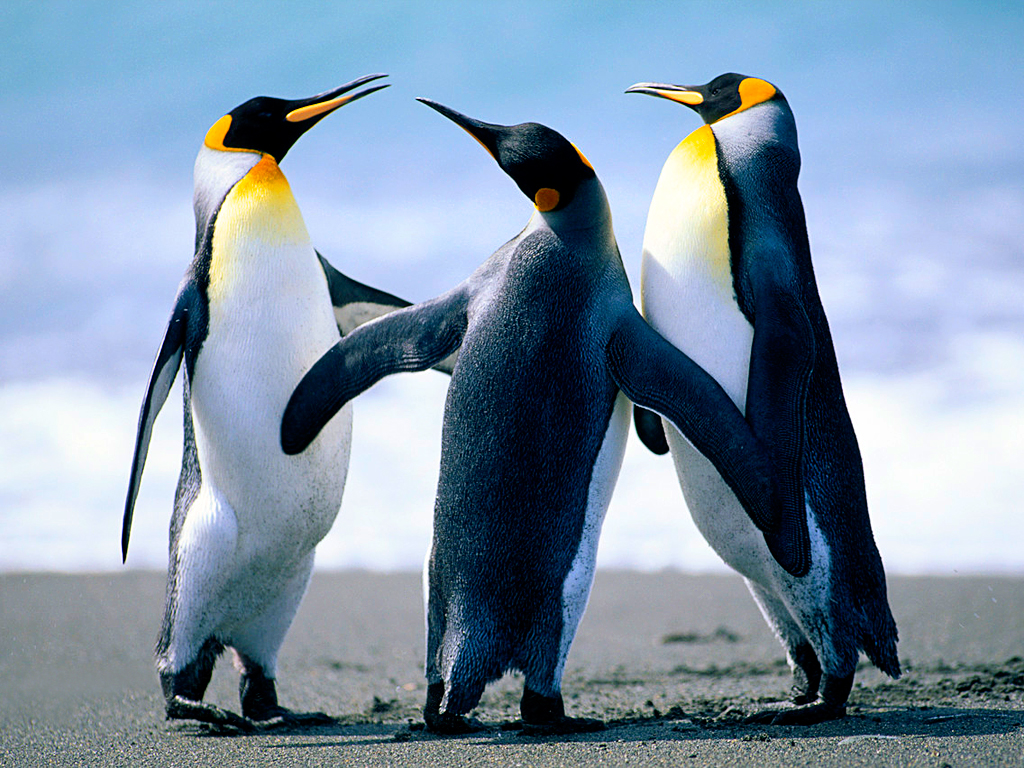
\includegraphics[scale=.50]{figures/Penguins.jpg}
%\caption{Another TAMU figure}
%\label{fig:tamu-fig4}
%\end{figure}
%%%%%%%%%%%%%%%%%%%%%%%%%%%%%%%%%%%%%%%%%%%%%%%%%%%%%%%

\subsection{Subsection}

%%%%%%%%%%%%%%%%%%%%%%%%%%%%%%%%%%%%%%%%%%%%%%%%%%%%%%%
%\begin{figure}[H]
%\centering
%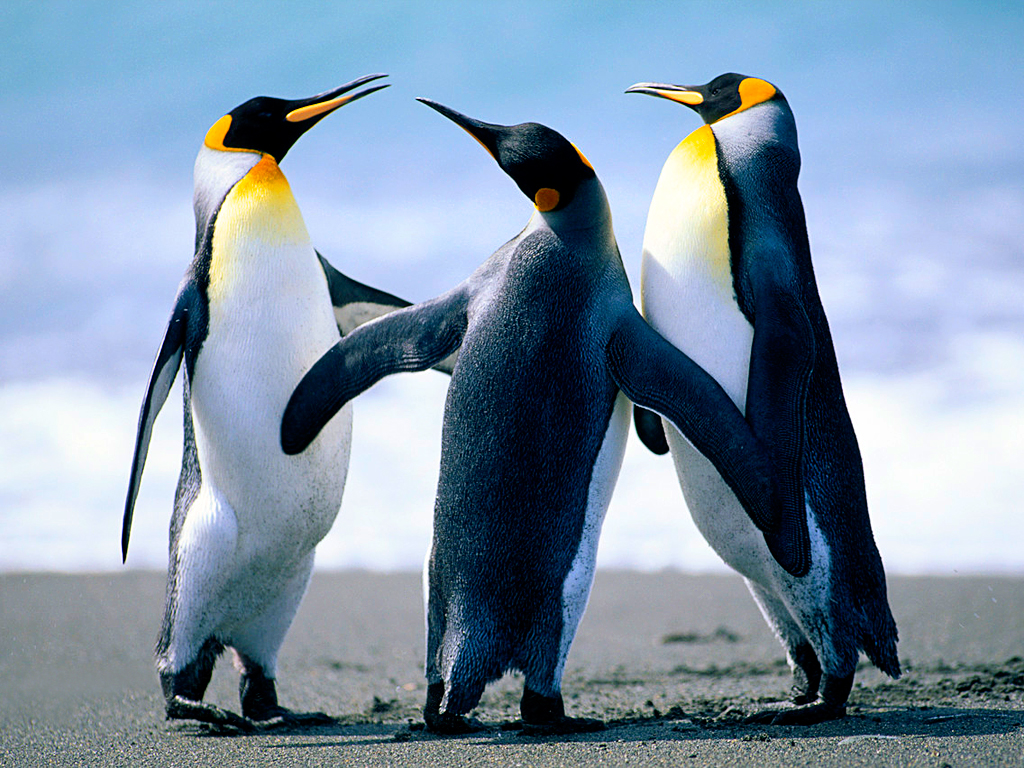
\includegraphics[scale=.50]{figures/Penguins.jpg}
%\caption{Another TAMU figure}
%\label{fig:tamu-fig4-2}
%\end{figure}
%%%%%%%%%%%%%%%%%%%%%%%%%%%%%%%%%%%%%%%%%%%%%%%%%%%%%%%
\subsection{Subsection}

A table example is going to follow.

\begin{table}[H]
\centering
\caption{This is a table template}
\begin{tabular}{|l|c|c|c|c|c|}
\hline
Product & 1 & 2 & 3 & 4 & 5\\
\hline
Price & 124.- & 136.- & 85.- & 156.- & 23.-\\
Guarantee [years] & 1 & 2 & - & 3 & 1\\
Rating & 89\% & 84\% & 51\% & & 45\%\\
\hline
\hline
Recommended & yes & yes & no & no & no\\
\hline
\end{tabular}
\label{tab:template2}
\end{table}
\section{Another Section}


\addcontentsline{toc}{part}{REFERENCES}
\renewcommand{\bibname}{{\normalsize\rm REFERENCES}}
\bibliographystyle{plain}
\bibliography{biblio}

\titleformat{\chapter}{\centering\normalsize}{APPENDIX \thechapter.}{1em}{}
\begin{appendices}
\renewcommand{\appendixname}{\uppercase{Appendix}}
%\renewcommand{\appendixtitle}{\uppercase{Appendix}}

\chapter[ ]{\uppercase{ML options}}

Some of the available coarsening schemes in ML \cite{ml_guide}:
\begin{description}
  \item[Uncoupled:] Attempt to construct aggregates of optimal size ($3^d$
    nodes in $d$ dimensions). Each process works independently and aggregates
    cannot span processes.
  \item[MIS:] Uses maximal independent set techniques to define aggregates.
    Aggregates can span processes. May provide better quality aggregates than
    {\bf Uncoupled}, but computationally more expensive because it requires
    matrix-matrix product.
\end{description}
Some of the smoothers:
\begin{description}
  \item[Jacobi]
  \item[Symmetric Gauss-Seidel]
\end{description}
Some of the coarse solvers:
\begin{description}
  \item[Jacobi]
  \item[Symmetric Gauss-Seidel]
  \item[Amesos-KLU:] Use {\bf KLU} through {\bf Amesos}. Coarse grid problem
    is shipped to processor 0, solved, and solution is broadcast.
  \item[Amesos-UMFPACK:] Use {\bf UMFPACK} through {\bf Amesos}. Coarse grid
    problem is shipped to processor 0, solved, and solution is broadcast.
  \item[Amesos-MUMPS:] Use double precision version of {\bf MUMPS} through
    {\bf Amesos}.
\end{description}
The MultiLevelPreconditioner class provide default values for five different
preconditioner types:
\begin{itemize}
  \item Classical smoothed aggregation for symmetric and positive definite or
    nearly symmetric and definite systems (used here)
  \item Classical smoothed aggregation-based two-level domain decomposition.
  \item Three-level algebraic domain decomposition.
  \item Eddy current formulation of Maxwell's equation.
  \item Energy-based minimizing smoothed aggregation suitable for highly
    convective nonsymmetric fluid flow problems.
\end{itemize}
The options used in this work are:
\begin{description}
  \item[option name:] SA
  \item[max levels:] 10
  \item[prec type:] $V-$cycle
  \item[aggregation type:] uncoupled-MIS
  \item[aggregation damping factor:] 4/3
  \item[eigen-analysis type:] cg
  \item[eigen-analysis iterations:] 10
  \item[smoother sweeps:] 2
  \item[smoother damping factor:] 1.0
  \item[smoother pre or post:] both
  \item[smoother type:] symmetric Gauss-Seidel
  \item[coarse type:] Amesos-KLU
  \item[coarse max size:] 128
\end{description}


\end{appendices}
\pagebreak{}



\end{document}
